\documentclass{article}
\usepackage[margin=1in]{geometry}
\usepackage{filecontents}
\usepackage[noadjust]{cite}
\usepackage{listings}
\usepackage{fancyvrb}
\usepackage{tabularx}
\usepackage{adjustbox}
\usepackage{textcomp}
%\usepackage{framed}
\usepackage[listings,skins]{tcolorbox}
\usepackage[skipbelow=\topskip,skipabove=\topskip]{mdframed}
\usepackage{makecell}
\usepackage{url}
\usepackage{tikz}
\usetikzlibrary{matrix,shapes,arrows,positioning}
\mdfsetup{roundcorner=0}

\graphicspath{ {images/} }

\begin{filecontents*}{bibi.bib}
@INBOOK {kubat,
    author    = "Miroslav Kubat",
    title     = "An Introduction to Machine Learning",
    chapter   = "Nearest Neighbor Classifiers",
    publisher = "Springer International",
    year      = "2017",
    edition   = "second"
}
@ONLINE {scikit,
    author = "Scikit-learn",
    title  = "Adaboost Classifier",
    url    = "http://scikit-learn.org/stable/modules/generated/sklearn.ensemble.AdaBoostClassifier.html"
}
@ONLINE {numpy,
    author  = "NumPy",
    title   = "NumPy Random Choice",
    url     = "https://docs.scipy.org/doc/numpy-1.13.0/reference/generated/numpy.random.choice.html"
    }
@ONLINE {ionosphere,
    title  = "Ionosphere Dataset",
    url    = "https://archive.ics.uci.edu/ml/datasets/ionosphere"
}
@ONLINE {cancer,
    title  = "Cancer Dataset",
    url    = "https://archive.ics.uci.edu/ml/datasets/breast+cancer+wisconsin+%28original%29"
}
@ONLINE {musk,
    title  = "Musk Dataset",
    url    = "https://archive.ics.uci.edu/ml/datasets/Musk+(Version+1)"
}
@CONFERENCE {sun-kamel-wang,
    author = "Yanmin Sun, Mohamed S. Kamel and Yang Wang",
    title = "Boosting for Learning Multiple Classes with Imbalanced Class Distribution",
    booktitle = "Data Mining, 2006. ICDM '06. Sixth International Conference on"
}
\end{filecontents*}   

\title{Voting Assemblies: Adaboost}
\author{Lloyd Beaufils, Jerry Bonnell, Gururaj Shriram}
\date{November 24, 2017}


\begin{document}
\maketitle

\section{Task}

Implement a basic version of \textit{Adaboost}. The number of voting classifiers is determined by a user-set constant. Another user-set constant specifies the number of examples in each training set, \textit{T\textsubscript{i}}. The weights of the individual classifiers are obtained with the help of \textit{perceptron learning}. Apply the program task to some of the benchmark domains from the UCI repository. Make observations about this program's performance on different data. For each domain, plot a graph showing how the overall accuracy of the resulting classifier depends on the number of subclassifiers. Also, observe how the error rate on the training set and the error rate on the testing set tend to converge with the growing number of classifiers.

\section{Introduction}

Adaboost is a machine learning meta-algorithm. It is a boosting algorithm derived from Schapire's boosting designed to minimize randomness and error. Schapire's Boosting seeks to minimize the randomness found in bagging, but it is often too strict and restrictive, and thus it is not often possible to find enough examples that satisfy its requirements. Adaboost takes the core idea of Schapire's boosting but examples are chosen probabilistically, allowing for a greater ease of selecting examples for the individual classifiers.

Adaboost creates classifiers one at a time, inducing each from a different training subset whose composition depends on the behavior of previous classifiers it has created. The training examples used are decided probabilistically as those on which the old classifiers would not perform well. Each example in the training set has a certain probability of being chosen, and those probabilities are altered with each induced classifier (examples that are repeatedly misclassified receive higher and higher probabilities). Another change from Schapire's boosting is that Adaboost does not stop at three classifiers- it induces a great many classifiers and makes the final decision with weighted majority voting between them.

\section{Method}

For this project, we implemented Adaboost in Python, using Table 9.3 in \cite{kubat}. Our Adaboost algorithm makes use of linear perceptron classifiers as the base classifiers. For the perceptron classifier, we again implemented our own version in Python (according to Table 4.1 in \cite{kubat}). To ensure that our Adaboost implementation was valid and reliably accurate, we tested it against a version from SciKit-learn, a popular machine learning library implemented in Python \cite{scikit}. \\

In Adaboost, the biggest innovation is that training sets for new classifiers are created probabilistically, with a preference for examples on which existing classifiers fail. This is achieved by selecting examples for the training sets with the aid of a mechanism known as the "wheel of fortune." This technique is known as the wheel of fortune because it can be visualized as follows: all the probabilities are placed on a wheel that is "spun." There is an indicator that lands within a probability range, and that example is selected for the current iteration. The actual implementation is equally straightforward- so long as the sum of probabilities is some number (i.e. 1), then generating a random number between 0 and that number will yield a single example. The probabilities of examples are continually added up, in order, and the first example whose probability causes sthe sum to exceed the random number is the one that is selected. This is repeated until the requisite number of examples are obtained, with obvious preference given to those examples with higher probability. In our project, we utilized a Python library called NumPy to do the random selection for us \cite{numpy}. Once all the requisite examples are chosen, a perceptron classifier is trained with them until the error rate reaches 5\% or less. \\

A key factor of the way Adaboost functions is with the updating of the probabilities of examples being chosen. This is done to allow for examples on which classifiers fail to have a higher chance of being selected for future classifiers. All examples start with equal probabilities, and the probabilities get updated after each new classifier is induced. For each example in the full training set that is correctly classified by the assembly after adding the \textit{i}-th classifier, its probability is multiplied by the term $\beta_i = \epsilon_i / (1 - \epsilon_i)$, where $\epsilon_i$ is the assembly's overall error on the entire training set. Therefore, the more examples that the classifier ensemble correctly labels, the smaller the value of $\beta$ and the smaller the reduction of the probabilities of the correctly classified examples. The probabilities of all examples are then normalized to 1 for selection of the next classifier. In short, examples that are correctly labeled are given an decrease in the probability to be chosen to train the next classifier, with the size of the decrease being proportional to the amount of misclassified examples. \\

Once all the subclassifiers have been induce, Adaboost can be used to classify examples in the testing set, and it does so with weighted majority voting. Each sub-classifier is given a weight according to its classification record- the higher the classifier's reliability, the larger its weight. These weights determine how much each classifier contributes to the final decision. The final classification is not decided by plain majority voting of the subclassifiers, as it is in Schapire's Boosting. Instead, all the weights of classifiers voting for the positive class are summed up, as are the weights for the negative classes, and then the class is decided by the larger of the two sums. \\

In our experiments, we varied the number of subclassifiers used in our final group classifier to see how it affected the accuracy. We measured the error rate on the testing and training sets starting with one classifier and going up to 50. We also compared Adaboost's error rate (with 1-50 subclassifiers) on the testing set with those of other classifiers- namely, decision trees and a single perceptron classifier. Our graphs highlighting our results can be found at the end of this document. For our tests, we used three datasets from the UCI machine learning repository- Ionosphere, Cancer, and Musk.

\section{Ionosphere Dataset}

The Ionosphere dataset was one obtained from the UCI machine learning repository \cite{ionosphere}. There are 34 continuous attributes and two class labels in this dataset. There are 351 examples and no missing values. The class distribution is 64.1\% positive / 35.9\% negative. \\

Adaboost performed remarkably well on the training set once it had at least 10 subclassifiers. The error rate dropped dramatically (from over 15\% to below 2.5\%) with the addition of the first ten classifiers, but then it reached a plateau of sorts. However, the error rate on the testing set did not change so dramatically with the variation of classifier numbers. After an initial spike above 17.5\%, the testing set error decreases and ends up dropping below 13\%. This shows the power of Adaboost- the assembly classifier ends up outperforming a single perceptron classifier trained on the entire training set. Also, it can handle the imbalanced classes present in this dataset as well, as noted in \cite{sun-kamel-wang}. The decision tree performed the best with an error rate of around 11\%. Our Adaboost never outperformed it. This is because decision trees simply do a better job of classifying this dataset. This is good, because it shows how, even though perceptron is a weaker classifier, its performance can definitely be improved with Adaboost.

\section{Cancer Dataset}

The Breast Cancer dataset was also obtained from the UCI repository \cite{cancer}. There are 10 discrete attributes and two class labels in this dataset. There are 683 examples and no missing attribute values (there were 16 examples with missing attribute values, but we removed them from the dataset for our experiments). The class distribution is 34.9\% positive / 65.1\% negative. \\

Like before, the error rate on the testing and training sets are observed to have a relatively sharp decrease with the addition of the first ten classifiers, which makes sense. Something to note is that the scale for the error rate is pretty small, so these changes are not as dramatic as they may seem. Adaboost performed better than a single perceptron classifier did when between around 20 and 30 subclassifiers, but then the error rate begins to rise again after that. This can be attributed to poor subclassifers being induced from outliers or other such noisy examples. The decision tree actually performed worse than a single perceptron or Adaboost did on this dataset, and that again points to noisy data, since decision trees are more succeptible to noise than Adaboost is. Another thing to note is that the classes in this dataset are imbalanced. As Adaboost is good at handling imbalanced classes \cite{sun-kamel-wang}, it performed well overall in bringing down the error rate, especially when the noise is taken into account.

\section{Musk Dataset}

Finally, the Musk data was also obtained from the UCI repository \cite{musk}. There are 168 discrete attributes and two class labels in this dataset. There are 476 examples and no missing attribute values. The class distribution is 43.4\% positive / 56.6\% negative. \\

Our Adaboost's performance on this dataset was a bit worse than its performance on the others, so we wanted to include this for completness' sake. As the graphs show, the error rate jumps up and down sharply with each new classifier. This is highly emblematic of noisy data and explains why our algorithm struggled with this dataset. The training set error slowly  decreases with the addition of the first twenty algorithms, as does the testing set error. However, the testing set error rises after reaching a minimum at around 23 examples. The decision tree struggled again, doing worse than Adaboost and showing that the data was noisy.

\section{Conclusion}

Our experiments show that Adaboost is successful at improving upon a base classifier's performance. With every test we made, Adaboost outperformed a single perceptron classifier with at least one specific number of classifiers. In noisy datasets, Adaboost struggles a bit more than a single perceptron, but it did still outperform it at least once in all of our experiments. When a dataset is not noisy, as with Ionosphere, Adaboost's error rate generally drops with the addition of more classifiers. We also find that our Adaboost performed well in datasets with imbalanced classes, a finding that is reinforced by \cite{sun-kamel-wang}. In our experiments, we did not observe the error rate on the training and testing sets converge; the training set error was always lower than the testing set's error. This is because the subclassifiers we used were perceptron, and the error rate cannot be reduced past a certain point. \\

\bibliographystyle{plainurl}
\bibliography{bibi} 

\begin{figure}[hbt]
\centering
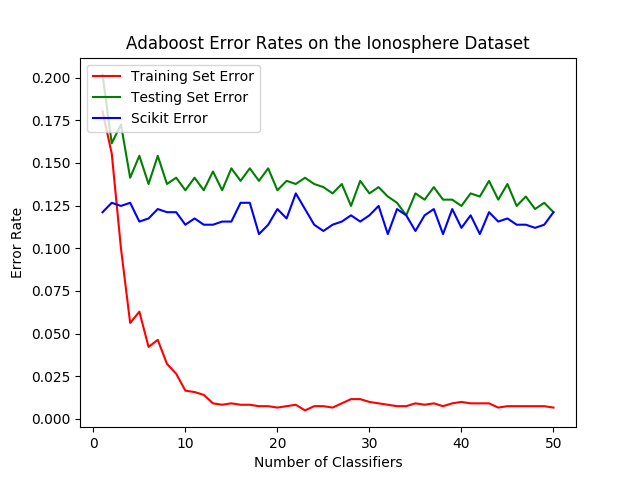
\includegraphics[scale=0.7]{Ionosphere_1}
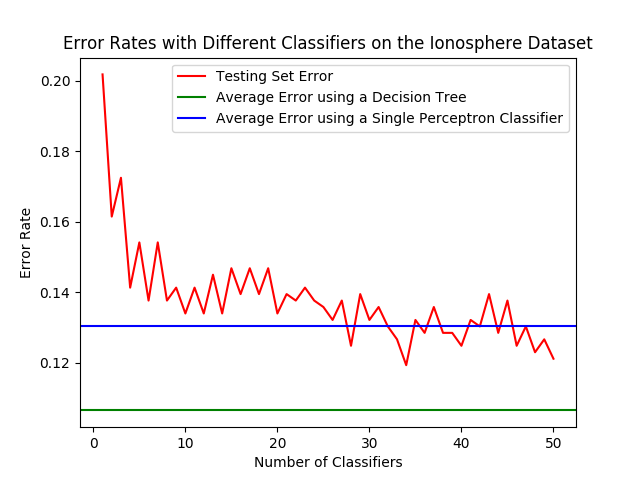
\includegraphics[scale=0.7]{Ionosphere_different_classifiers_1} 
\caption{The error rate on the testing and training sets drop dramatically with the first 10 classifiers. Adaboost does slightly better than a single perceptron classifier and consistently worse than a decision tree. The testing set error generally decreases with more subclassifiers, approaching the decision tree's accuracy.}
\end{figure}

\begin{figure}[hbt]
\centering
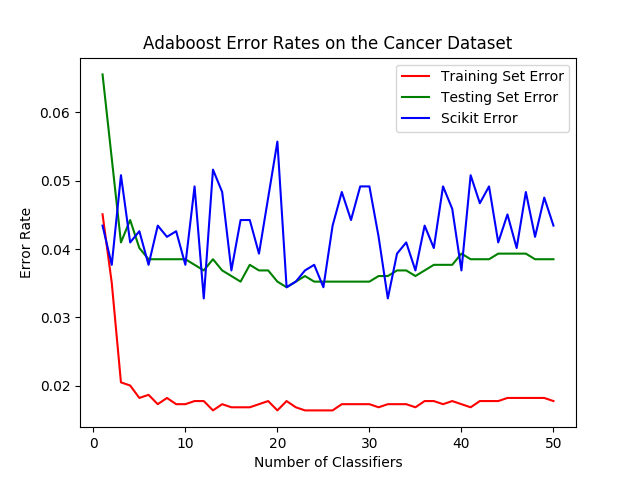
\includegraphics[scale=0.7]{Cancer_1}
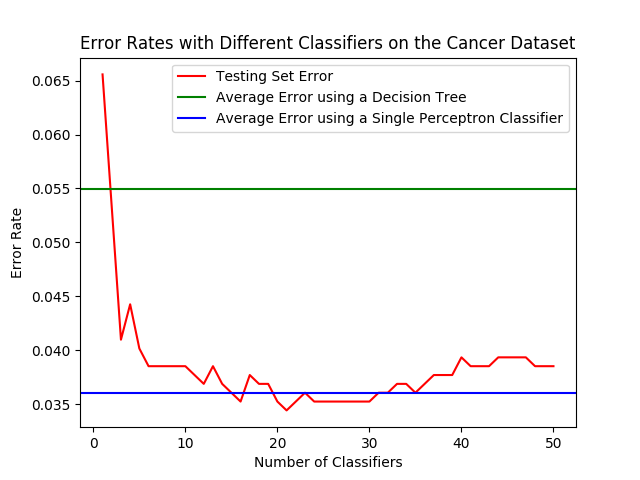
\includegraphics[scale=0.7]{Cancer_different_classifiers_1} 
\caption{The testing and training set errors here experience an even sharper relative decline. The dataset is noisy, leading the decision tree to do worse than Adaboost and the single perceptron. After hitting a minimum between 20 and 30 examples, the testing set error rate begins to climb back up again due to the noise in the data and bad examples being chosen to induce subclassifiers.}
\end{figure}

\begin{figure}[hbt]
\centering
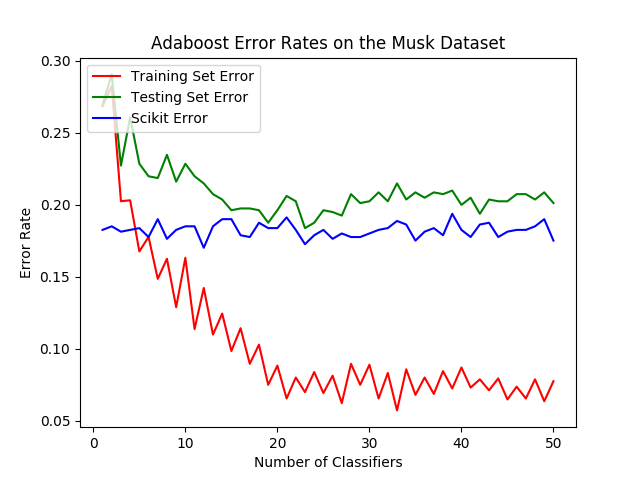
\includegraphics[scale=0.7]{Musk_1}
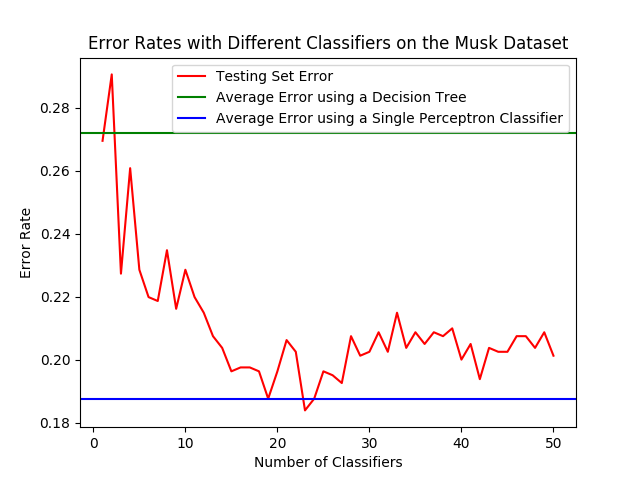
\includegraphics[scale=0.7]{Musk_different_classifiers_1} 
\caption{The data here is especially noisy, causing the training set error rate to jump up and down erratically. The testing set error does not fare much better, reaching a minimum around 23 and climbing back up past the error rate of a single perceptron classifier. The decision tree also suffers due to the noise in the data.}
\end{figure}


\end{document}
